\newpage
\appendix
\section{Appendix} \label{appendix}
\pagenumbering{roman}
\begin{figure}[H]
    \centering
    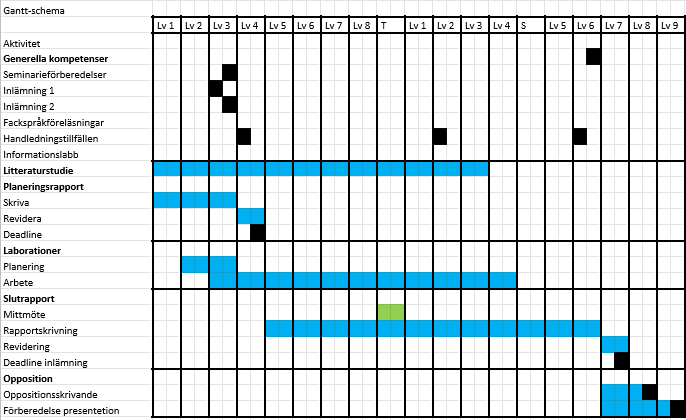
\includegraphics[scale=0.8]{Ganttliten.PNG}
    \caption{Gantt-schema över veckorna relaterat till projektbeskrivningen}
    \label{fig:Ganttliten}
\end{figure}

\newpage
\thispagestyle{empty}
\begin{figure}[H]
    \centering
    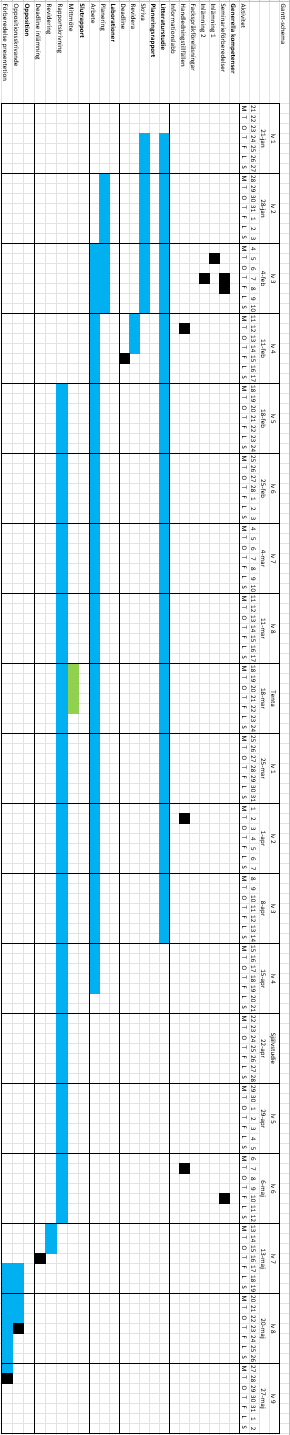
\includegraphics[scale=0.6]{Ganttroterad.PNG}
    \caption{Gantt-schema över hela projektet, dag för dag}
    \label{fig:Ganttroterad}
\end{figure}
\newpage
\thispagestyle{empty}
\begin{figure}[H]
    \centering
    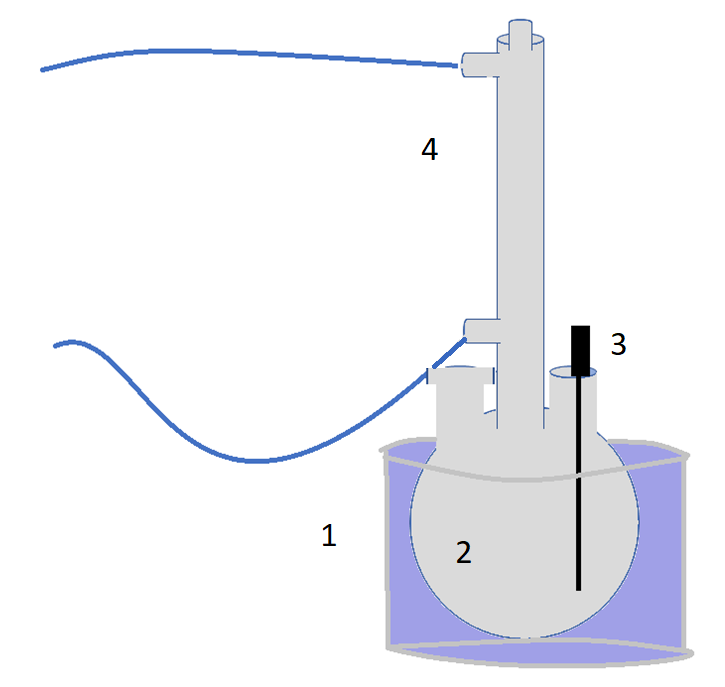
\includegraphics[scale=0.6]{labbupp.png}
    \caption{Laborations uppställningen i nuläget. 1. Vattenbad som värms upp med en värmeplatta. 2. Trehalsad rundbottenskolonn. 3. Termometer som är kopplad till värmeplatten. 4. Kondensor.    }
    \label{fig:lab}
\end{figure}

\newpage
\thispagestyle{empty}
\begin{figure}[H]
    \centering
    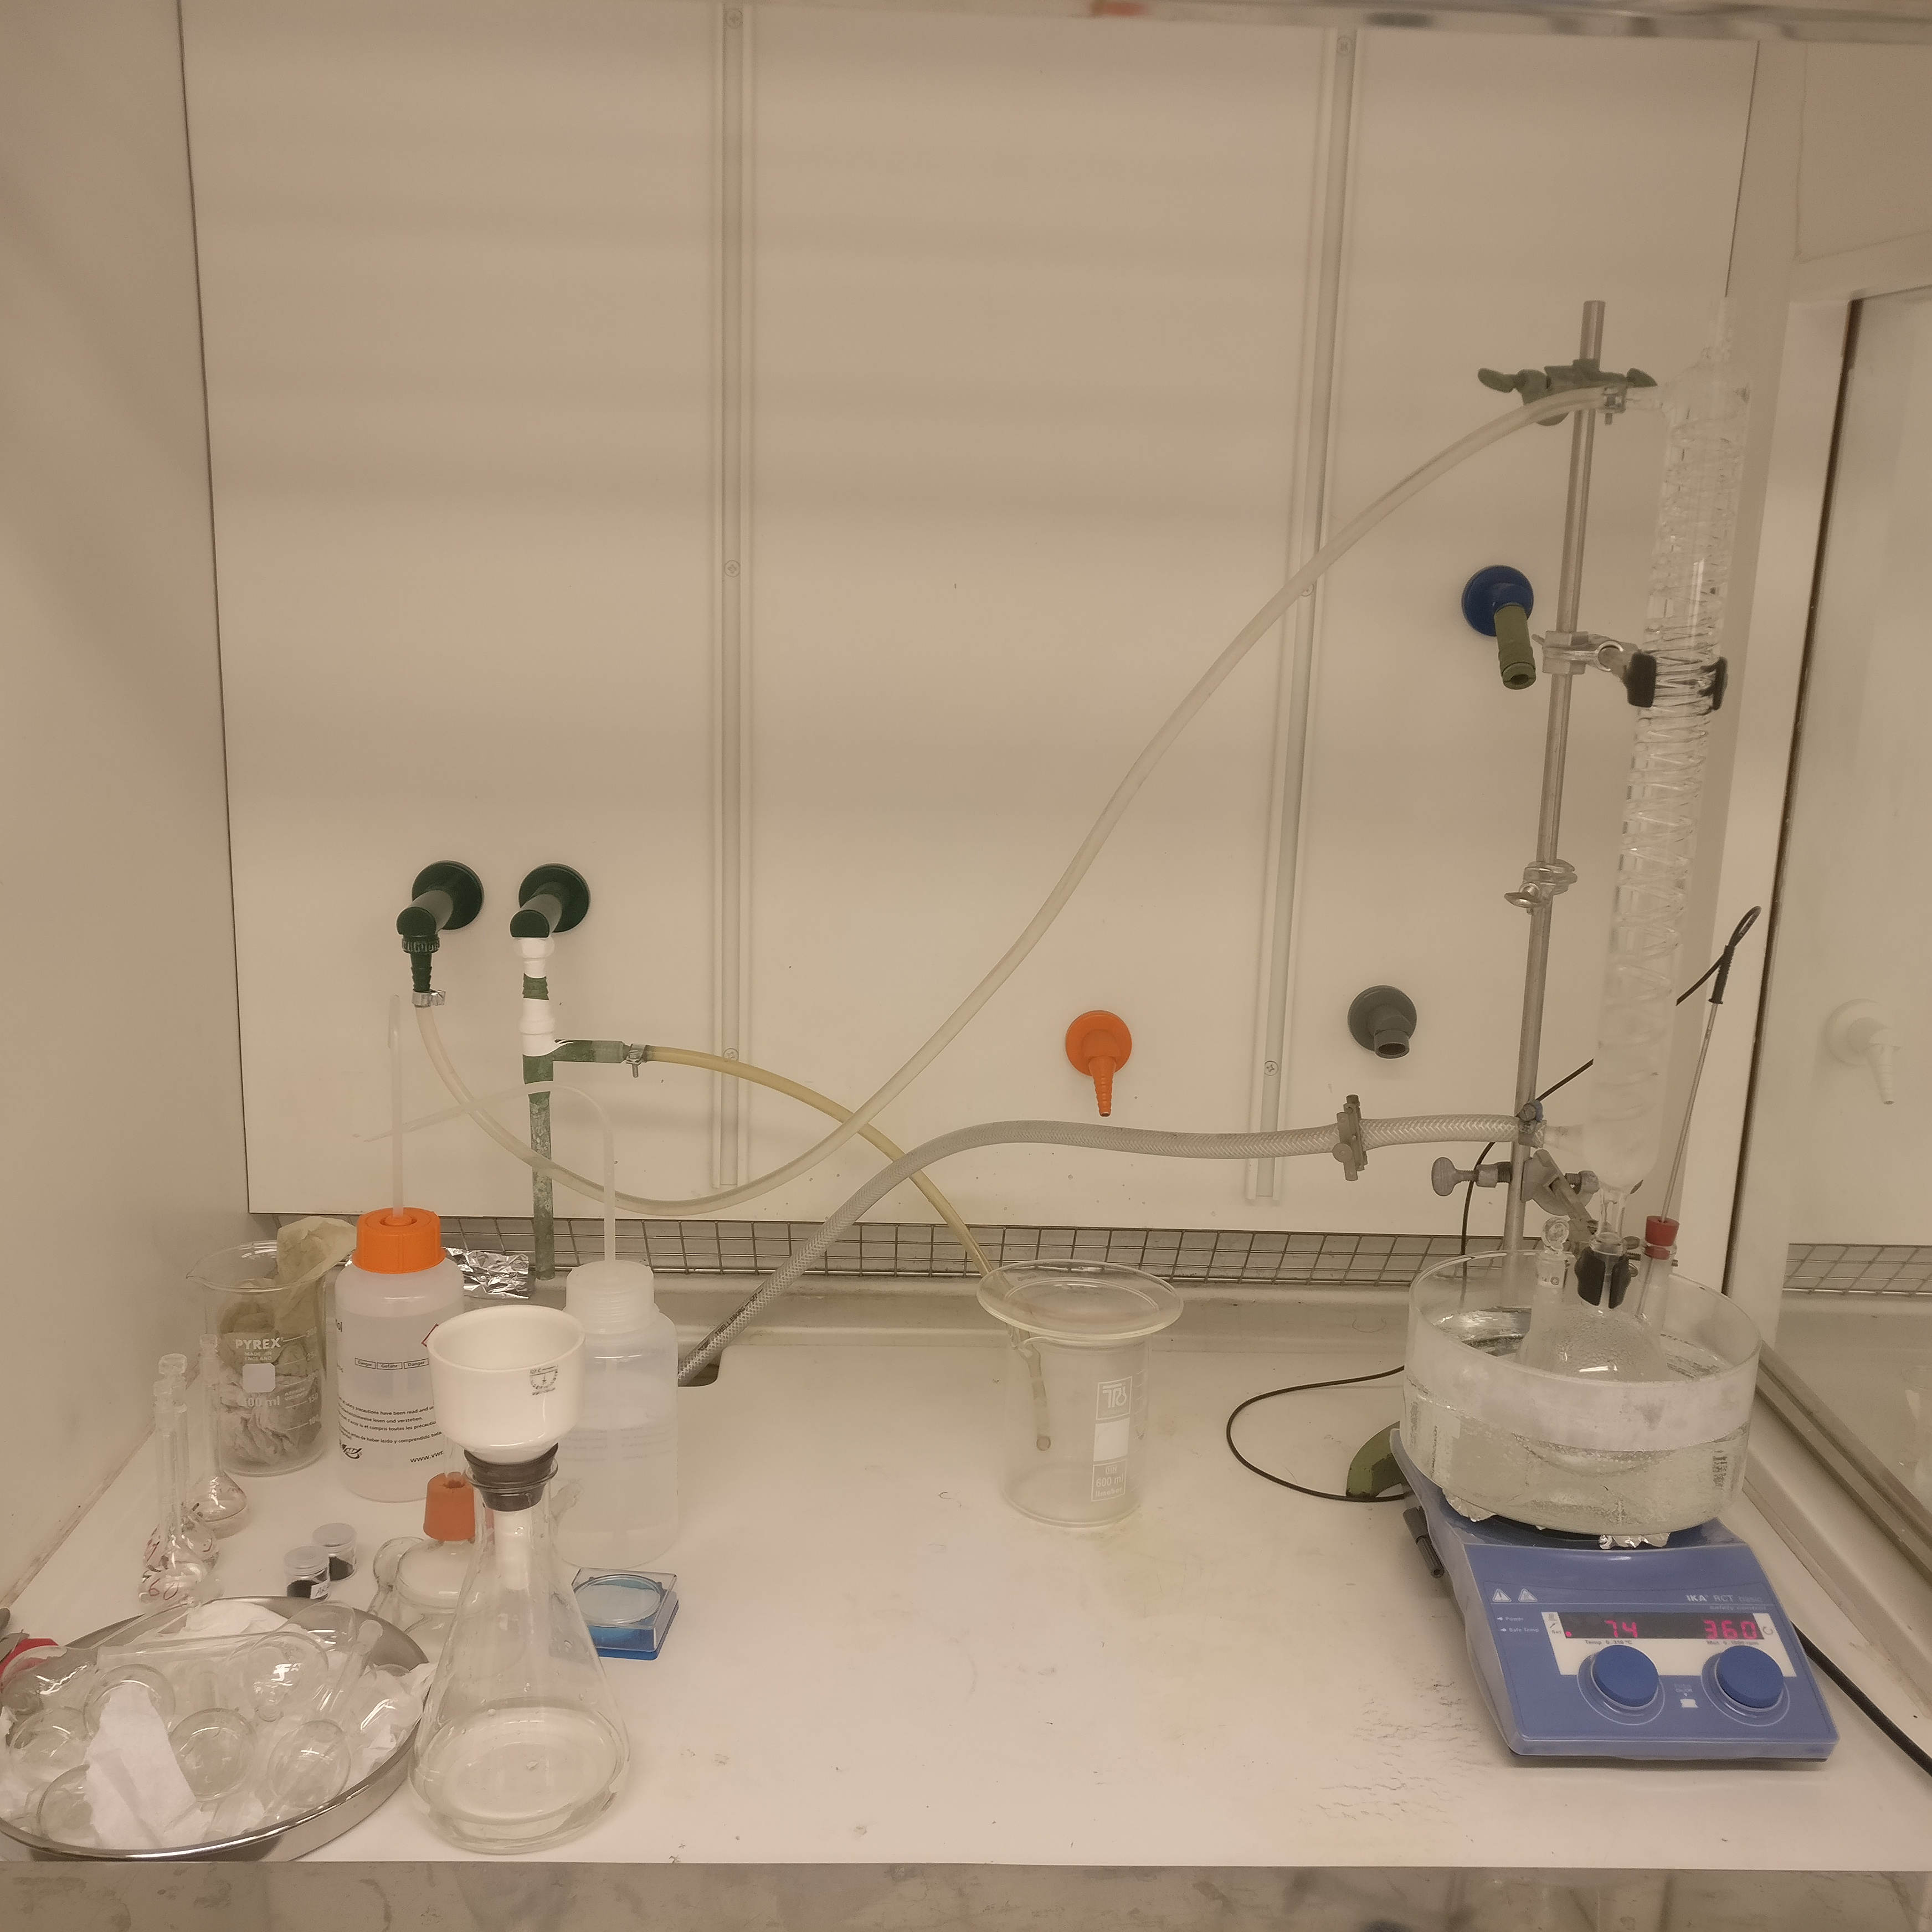
\includegraphics[scale=0.1]{labsetup.jpg}
    \caption{Laborations uppställningen i nuläget.}
    \label{fig:labpaint}
\end{figure}



